\documentclass[a4paper, 12pt]{exam}

% Exam class is broken without this.
\makeatletter
\expandafter\providecommand\expandafter*\csname ver@framed.sty\endcsname
{2003/07/21 v0.8a Simulated by exam}
\makeatother

% Enables the use of colour.
\usepackage{xcolor}
% Syntax high-lighting for code. Requires Python's pygments.
\usepackage{minted}
% Enables the use of umlauts and other accents.
\usepackage[utf8]{inputenc}
% Diagrams.
\usepackage{tikz}
% Settings for captions, such as sideways captions.
\usepackage{caption}
% Symbols for units, like degrees and ohms.
\usepackage{gensymb}
% Latin modern fonts - better looking than the defaults.
\usepackage{lmodern}
% Allows for columns spanning multiple rows in tables.
\usepackage{multirow}
% Better looking tables, including nicer borders.
\usepackage{booktabs}
% More math symbols.
\usepackage{amssymb}
% More math layouts, equation arrays, etc.
\usepackage{amsmath}
% More math fonts, like mathbb.
\usepackage{amsfonts}
% More theorem environments.
\usepackage{amsthm}
% More column formats for tables.
\usepackage{array}
% Adjust the sizes of box environments.
\usepackage{adjustbox}
% Better looking single quotes in verbatim and minted environments.
\usepackage{upquote}
% URLs.
\usepackage[hidelinks]{hyperref}
% Better blank space decisions.
\usepackage{xspace}
% Better looking tikz trees.
\usepackage{forest}
% For plotting.
\usepackage{pgfplots}

% Various tikz libraries.
\usetikzlibrary{mindmap}
\usetikzlibrary{shadows}
\usetikzlibrary{arrows}
\usetikzlibrary{positioning}
\usetikzlibrary{chains}
\usetikzlibrary{fit}
\usetikzlibrary{shapes}
\usetikzlibrary{decorations.markings}
\usetikzlibrary{calc}
\usetikzlibrary{arrows.meta}

% GMIT colours.
\definecolor{gmitblue}{RGB}{20,134,225}
\definecolor{gmitred}{RGB}{220,20,60}
\definecolor{gmitgrey}{RGB}{67,67,67}

% Rename Bibliography to a smaller "Refereces".
\renewcommand{\refname}{\selectfont\normalsize References} 

% Stop minted high-lighting errors.
\makeatletter
\expandafter\def\csname PYGdefault@tok@err\endcsname{\def\PYGdefault@bc##1{{\strut ##1}}}
\makeatother

% Set the header and footer.
\pagestyle{headandfoot}
\header{\textbf{Problem Sheet: Algorithms}}{}{Graph Theory}
\footer{}{Page \thepage\ of \numpages}{}

% Change some things to do with marks.
\marksnotpoints
\pointsinrightmargin

% Empty cover page.
\begin{coverpages}
\end{coverpages}

% Print answers
% \printanswers

\begin{document}

\begin{questions}

\question
  Re-write each of the following infix expressions in reverse Polish notation, evaluate them using the stack method and draw evaluation trees representing them.
  \begin{parts}
    \part $3 + 4$
    \part $3 + 4 \times 5$
    \part $(3 + 4) \times 5$
    \part $5 + 4 \times (6 \div 3)$
    \part $((16 \times 2) + 100) \div (11 \times 3) \times 75$
  \end{parts}

  \begin{solution}
    \begin{parts}
      \part
        $4 \quad 3 \quad + $
        \begin{center}
          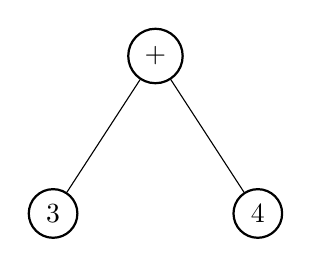
\begin{tikzpicture}[level/.style={level distance = 2cm},level 1/.style={sibling distance=26mm},level 2/.style={sibling distance=8mm}]
            \begin{scope}[every node/.style={circle,thick,draw}]
              \node {$+$}
                child { node {$3$} }
                child { node {$4$} };
            \end{scope}
          \end{tikzpicture}
        \end{center}

      \part
        $5 \quad 4 \quad \times \quad 3 \quad + $
        \begin{center}
          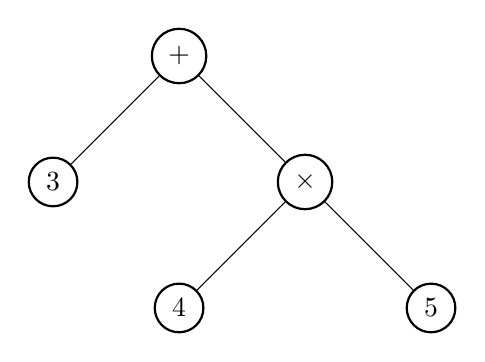
\begin{tikzpicture}[level/.style={level distance = 16mm},level 1/.style={sibling distance=32mm},level 2/.style={sibling distance=32mm}, level 3/.style={sibling distance=16mm},level 4/.style={sibling distance=16mm}]
            \begin{scope}[every node/.style={circle,thick,draw}]
              \node {$+$}
                child { node {$3$} }
                child { node {$\times$}
                  child { node {$4$} }
                  child { node {$5$} }
                };
            \end{scope}
          \end{tikzpicture}
        \end{center}

      \part
        $5 \quad 4 \quad 3 \quad + \quad \times $
        \begin{center}
          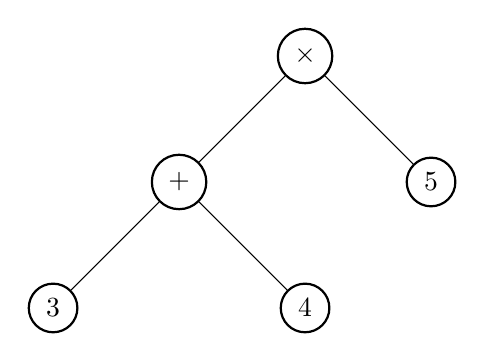
\begin{tikzpicture}[level/.style={level distance = 16mm},level 1/.style={sibling distance=32mm},level 2/.style={sibling distance=32mm}, level 3/.style={sibling distance=16mm},level 4/.style={sibling distance=16mm}]
            \begin{scope}[every node/.style={circle,thick,draw}]
              \node {$\times$}
                child { node {$+$}
                  child { node {$3$} }
                  child { node {$4$} }
                }
                child { node {$5$} };
            \end{scope}
          \end{tikzpicture}
        \end{center}

      \part
        $3 \quad 6 \quad  \div \quad 4 \quad 5 \quad + \quad \times $
        \begin{center}
          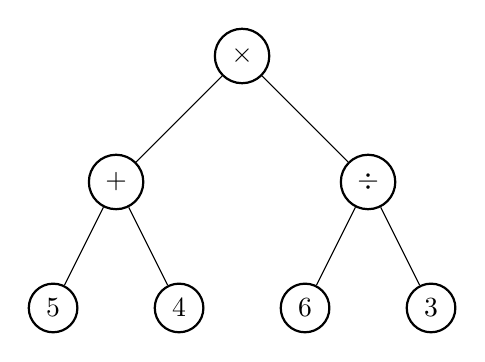
\begin{tikzpicture}[level/.style={level distance = 16mm},level 1/.style={sibling distance=32mm},level 2/.style={sibling distance=16mm}, level 3/.style={sibling distance=16mm},level 4/.style={sibling distance=16mm}]
            \begin{scope}[every node/.style={circle,thick,draw}]
              \node {$\times$}
                child { node {$+$}
                  child { node {$5$} }
                  child { node {$4$} }
                }
                child { node {$\div$}
                  child { node {$6$} }
                  child { node {$3$} }
                };
            \end{scope}
          \end{tikzpicture}
        \end{center}

      \part
        $75 \quad 3 \quad 11 \quad \times \quad 100 \quad 2 \quad 16 \quad \times \quad + \quad \div \quad \times$
        \begin{center}
          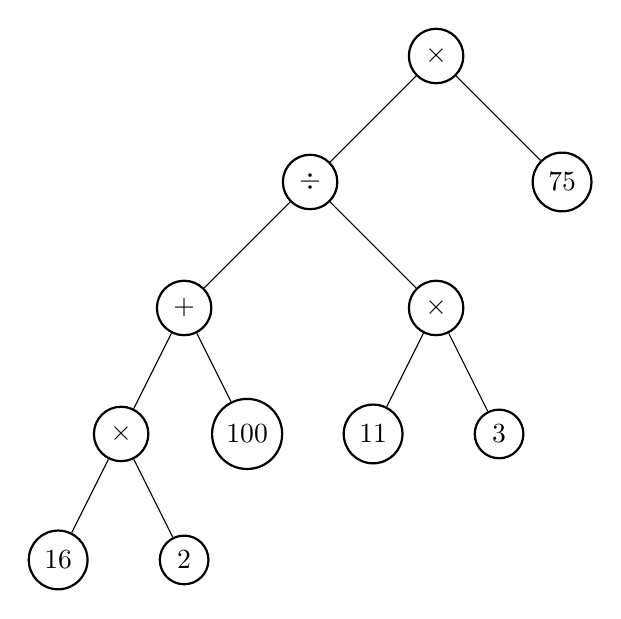
\begin{tikzpicture}[level/.style={level distance = 16mm},level 1/.style={sibling distance=32mm},level 2/.style={sibling distance=32mm}, level 3/.style={sibling distance=16mm},level 4/.style={sibling distance=16mm}]
            \begin{scope}[every node/.style={circle,thick,draw}]
              \node {$\times$}
                child { node {$\div$}
                  child { node {$+$}
                    child { node {$\times$}
                      child { node {$16$} }
                      child { node {$2$} }
                    }
                    child { node {$100$} }
                  }
                  child { node {$\times$}
                    child { node {$11$} }
                    child { node {$3$} }
                  }
                }
                child { node {$75$} };
            \end{scope}
          \end{tikzpicture}
        \end{center}
    \end{parts}
  \end{solution}

\question
  Draw a ternary decision tree of height at most two, representing the following problem.

  Suppose you have access to the international prototype kilogram.
  This is a weight, kept in France, which is the definition of the kilogram.
  You are presented with four other weights which are supposed to each be exactly one kilogram.
  However, you suspect that one of them is not a kilogram in weight but you can't tell which one it is.
  You don't have access to a weighing scales, but you do have access to a balance.
  This balance can be used to compare the weights of various objects and combinations of objects.~\cite{biggs02}
  
  \begin{solution}
    \begin{center}
      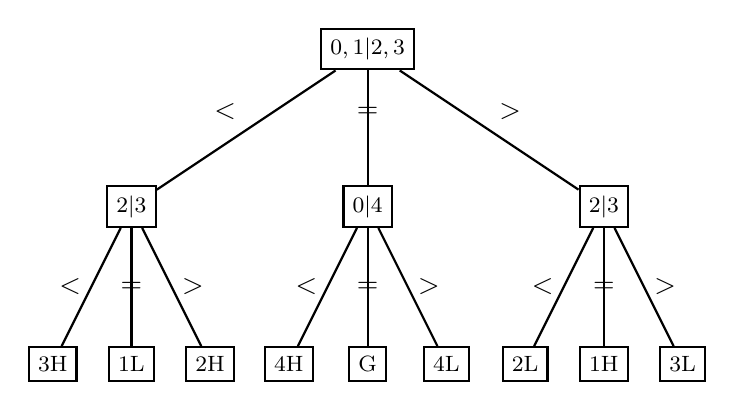
\begin{tikzpicture}
        \begin{scope}[every node/.style={thick,draw}]
          \node (a) at (0,4) {\footnotesize $0,1 | 2,3$};
          \node (b) at (-3,2) {\footnotesize $2 | 3$};
          \node (c) at (0,2) {\footnotesize $0 | 4$};
          \node (d) at (3,2) {\footnotesize $2 | 3$};
          \node (e) at (-4,0) {\footnotesize 3H};
          \node (f) at (-3,0) {\footnotesize 1L};
          \node (g) at (-2,0) {\footnotesize 2H};
          \node (h) at (-1,0) {\footnotesize 4H};
          \node (i) at (0,0) {\footnotesize G};
          \node (j) at (1,0) {\footnotesize 4L};
          \node (k) at (2,0) {\footnotesize 2L};
          \node (l) at (3,0) {\footnotesize 1H};
          \node (m) at (4,0) {\footnotesize 3L};
        \end{scope}
        \begin{scope}[every edge/.style={draw=black,thick}]
          \path (a) edge node[above left] {$<$}  (b);
          \path (a) edge node[above] {$=$}  (c);
          \path (a) edge node[above right] {$>$} (d);
          \path (b) edge node[left] {$<$}  (e);
          \path (b) edge node[] {$=$}  (f);
          \path (b) edge node[right] {$>$} (g);
          \path (c) edge node[left] {$<$}  (h);
          \path (c) edge node[] {$=$}  (i);
          \path (c) edge node[right] {$>$} (j);
          \path (d) edge node[left] {$<$}  (k);
          \path (d) edge node[] {$=$}  (l);
          \path (d) edge node[right] {$>$} (m);
        \end{scope}
      \end{tikzpicture}
    \end{center}
  \end{solution}

\question
  Draw a decision tree for bubble sort with three elements.~\cite{biggs02}
  \begin{solution}
    \begin{center}
      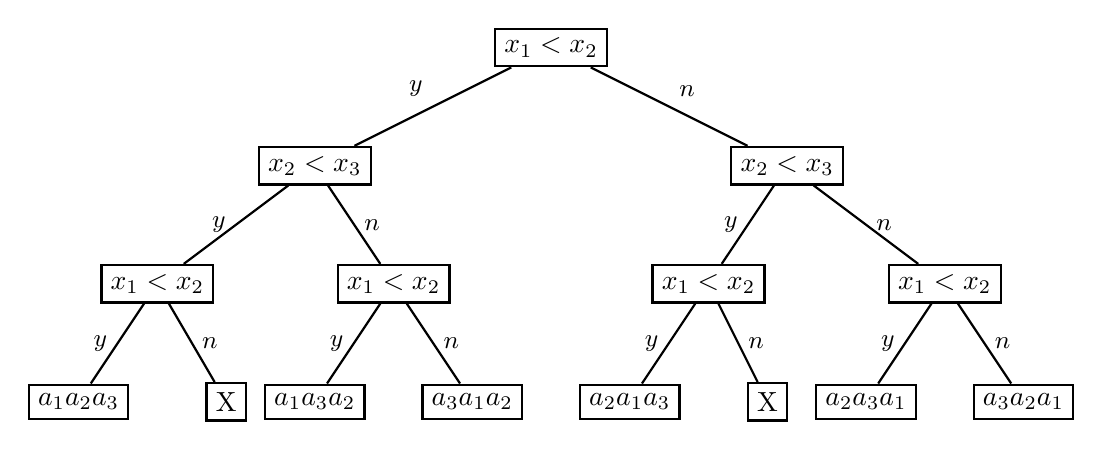
\begin{tikzpicture}
        \begin{scope}[every node/.style={thick,draw}]
          \node (a) at (4,6) {$x_1 < x_2$};
          \node (b) at (1,4.5) {$x_2 < x_3$};
          \node (c) at (7,4.5) {$x_2 < x_3$};
          \node (d) at (-1,3) {$x_1 < x_2$};
          \node (e) at (2,3) {$x_1 < x_2$};
          \node (f) at (6,3) {$x_1 < x_2$};
          \node (g) at (9,3) {$x_1 < x_2$};
          \node (h) at (-2,1.5) {$a_1 a_2 a_3$};
          \node (i) at (-0.125,1.5) {X};
          \node (j) at (1,1.5) {$a_1 a_3 a_2$};
          \node (k) at (3,1.5) {$a_3 a_1 a_2$};
          \node (l) at (5,1.5) {$a_2 a_1 a_3$};
          \node (m) at (6.75,1.5) {X};
          \node (n) at (8,1.5) {$a_2 a_3 a_1$};
          \node (o) at (10,1.5) {$a_3 a_2 a_1$};
        \end{scope}
        \begin{scope}[every edge/.style={draw=black,thick}]
          \path (a) edge node[above left] {\small $y$} (b);
          \path (a) edge node[above right] {\small $n$} (c);
          \path (b) edge node[left] {\small $y$} (d);
          \path (b) edge node[right] {\small $n$} (e);
          \path (c) edge node[left] {\small $y$} (f);
          \path (c) edge node[right] {\small $n$} (g);
          \path (d) edge node[left] {\small $y$} (h);
          \path (d) edge node[right] {\small $n$} (i);
          \path (e) edge node[left] {\small $y$} (j);
          \path (e) edge node[right] {\small $n$} (k);
          \path (f) edge node[left] {\small $y$} (l);
          \path (f) edge node[right] {\small $n$} (m);
          \path (g) edge node[left] {\small $y$} (n);
          \path (g) edge node[right] {\small $n$} (o);
        \end{scope}
      \end{tikzpicture}
    \end{center}
  \end{solution}



\question
  What is the smallest possible height of the decision tree of an algorithm for sorting four objects using binary comparisons?~\cite{biggs02}

  \begin{solution}
    Number of outcomes (leaves) is $l = 4! = 24$.
    Binary tree, so $m = 2$.
    So minimum height is $log_2 24 \approx 4.58$.
    Rounding up, gives smallest height as 5.
  \end{solution}

\question
  Calculate the minimum number of binary comparisons needed (in the worst case) when four objects are sorted by bubble sort.~\cite{biggs02}.
  \begin{solution}
    $3 + 2 + 1 = 6$
  \end{solution}

\end{questions}

\bibliographystyle{plain}
\bibliography{bibliography}

\end{document}
